\title{\vspace{160px} \textbf{\huge{Multimedia}} \\\vspace{17.5px} \LARGE{Homework 2}  \vspace{10px}}
\author{\href{https://github.com/imAlessas}{Alessandro Trigolo}}
\date{7 Giugno 2024}

\begin{document}

\maketitle\newpage

\tableofcontents
\vspace{50px}
\listoffigures
\newpage


\section{Introduzione}

Il seguente documento ha l'obiettivo di mostrare la procedura attuata per analizzare le prestazioni di una rete, in particolare di un collegamento tra un \textsl{host} ed un server seguendo le indicazione dell'homework. A tal scopo verrà illustrato e spiegato lo script necessario per effettuare questo tipo di analisi. 

In particolare, l'analisi si divide in tre principali parti. La prima ha l'obiettivo di recuperare il numero di connessioni che separano l'host con il server (paragrafo\,\ref{links}). In secondo luogo al server verrà mandata una elevata quantità di pacchetti con dimensioni diverse al fine di ottenere la latenza tra la sorgente e la destinazione, ovvero il Round Trip Time (vedi\,\ref{RTT}). Infine, con tutti i dati recuperati sarà possibile modellare la distribuzione di latenze con l'obiettivo di ottenere il throughput (sezione\,\ref{throughput}).

\vspace{10px}\subsection{Utilizzo dello script}

Le richieste dell'homework sono state soddisfatte attraverso uno script scritto con il linguaggio \textsl{Python} ed eseguito sul sistema operativo \textsl{Windows 10} in lingua italiana. Tutte le richieste sono state soddisfatte attraverso l'utilizzo del comando \texttt{ping} che si occupa di inviare delle richieste ICMP\footnote{ICMP sta per \textsl{Internet Control Message Protocol} è un protocollo utilizzato dai dispositivi di una rete per comunicare la presenza di problemi riguardanti la trasmissione dei dati} ad una determinata destinazione. La risposta del suddetto comando diagnostico è il periodo impiegato dalla destinazione per rispondere, ovvero la \textbf{latenza}.

Prima di lanciare lo script, è necessario aprire il file \textsl{script.py} e impostare correttamente il percorso dello script modificando la costante \texttt{PATH\_TO\_SCRIPT}.
\begin{lstlisting}
    PATH_TO_SCRIPT = os.path.join("multimedia", "hw-2", "script")
\end{lstlisting}

\noindent In secondo luogo è possibile impostare le specifiche di progetto mediante delle costanti che indicano il nome del server su cui inviare le richieste, il numero di instanze da mandare ad ogni richiesta ping e l'incremento di lunghezza (step) che ci sarà tra la lunghezza del pacchetto durante l'iterazione \textit{i} e la successiva \textit{i + 1}.

\begin{lstlisting}
    # project specification
    SELECTED_SERVER_CITY = "Atlanta"
    INSTANCES = 30
    STEP_BETWEEN_LENGTHS = 25
\end{lstlisting}

\noindent Tali impostazioni verranno poi brevemente processate con il seguente codice. In particolare si osserva che la costante \texttt{SELECTED\_SERVER\_CITY} verrà utilizzata per ottenere l'effettivo dominio del server e l'abbreviazione del nome della città. In secondo luogo la costante \texttt{STEP\_BETWEEN\_LENGTHS} verrà utilizzata per generare un vettore che parta da 10 e per arrivare a 1471 incrementa il suo valore di esattamente \texttt{STEP\_BETWEEN\_LENGTHS}.

\begin{lstlisting}
    SERVERS = {
        "Atlanta" : "atl.speedtest.clouvider.net",
        "New York City" : "nyc.speedtest.clouvider.net", 
        "London" : "lon.speedtest.clouvider.net", 
        "Los Angeles" : "la.speedtest.clouvider.net", 
        "Paris" : "paris.testdebit.info", 
        "Lillie" : "lille.testdebit.info", 
        "Lyon" : "lyon.testdebit.info", 
        "Aix-Marseille" : "aix-marseille.testdebit.info", 
        "Bordeaux" : "bordeaux.testdebit.info"
    }

    # set choosen options
    server = SERVERS[SELECTED_SERVER_CITY]
    city = server.split(".")[0]
    payload_lengths = range(10, 1471, STEP_BETWEEN_LENGTHS)
\end{lstlisting}

\noindent Usando le impostazioni dell'esempio, lo script — che sarà descritto nel capitolo\,\ref{performance} — manderà le richieste al server di Atlanta \texttt{atl.speedtest.clouvider.net}. Lo script poi, al fine di analizzare le performance di rete di tale server, per ogni valore di lunghezza all'interno della lista \texttt{payload\_lengths}, effettureà 30 istanze di richiesta. In altre parole si faranno 30 richieste di lunghezza 10 byte al server di Atlanta, poi altre 30 di lunghezza 10 + 25 = 35 byte, poi altre 30 di lunghezza 35 + 25 = 60 bytes e così via fino ad arrivare alla lunghezza 1470 bytes, per un totale di 1770 richieste.



\vspace{10px}\subsection{Parametri di progetto}

All'interno dello script vegono utilizzati due tipi di comando \texttt{ping}. Il primo, utilizzato nella prima task, descritta nel paragrafo\,\ref{links}, è il comando ping di default di Windows: lo script funziona solo e soltanto se la lingua di Windows è in italiano altrimenti non è possibile analizzare correttamente le risposte del comando. Nella seconda task, esplorata nel paragrafo\,\ref{RTT}, viene utilizzato invece il comando \texttt{psping}, che è in lingua inglese. Al fine di riuscre ad utilizzare lo script è necessari avere l'eseguibile \texttt{psping.exe} all'interno della cartella da cui poi viene eseguito lo script (ovvero la cartella che, attraverso il percorso all'interno di \texttt{PATH\_TO\_SCRIPT}, permette di arrivare al file \texttt{script.py}). Si è scelto di utilizzare psping in quanto è più prestante del comando ping di default. Inoltre nel primo punto non si è utilizzato psping in quanto non è presente l'impostazione che permette di ridurre il Time-To-Live del pacchetto.

In secondo luogo, al fine di eseguire i comandi nel terminale, non si è utilizzata la funzione \texttt{os.system}, bensì la libreria \texttt{subprocess}, 
che permette di ottenere il risultato direttemane in una stringa senza avere la necessità di scriverlo sul file per poi accedere al file per leggerlo. Questo migliora le prestazioni computazionali dello script, in particolare nella seconda parte dove in genere viene inviata una mole elevata di pacchetti ICMP. È comunque possible scrivere su files i risultati dell'esecuziuone del comando, è sufficiente impostare a \texttt{True} la \textsl{flag} che si chiama \texttt{SAVE\_TO\_FILE}.

Le analisi che seguiranno saranno effettutate sul server di Los Angeles il cui dominio è \texttt{la.speedtest.clouvider.net}. In particolare verranno prese in considerazione tre diverse istanze di esecuzione dello script, le quali avranno un numero crescente di pacchetti da mandare:

\begin{enumerate}
    \setlength{\itemsep}{4px}
    \item 20 messaggi ed uno step di 10, quindi un totale di 2940 pacchetti (figure\,\ref{fig:20-instances-total},\,\ref{fig:20-instances-stats},\,\ref{fig:20-instances-min});
    \item 100 instanze ed uno step di 2, ammontando a 73100 blocchi (figure\,\ref{fig:100-instances-total},\,\ref{fig:100-instances-stats},\,\ref{fig:100-instances-min});
    \item 250 pacchetti ed uno step di 1, per un totale di 365250 messaggi (figure\,\ref{fig:250-instances-total},\,\ref{fig:250-instances-stats},\,\ref{fig:250-instances-min}).
\end{enumerate}



\newpage\section{Performance di rete}\label{performance}

Dopo aver introdotto i parametri di progetto adottati, andremo ora ad analizzare le perfomrance di rete. In particolare ci occupiamo di analizzare il numero di connessione che debbono essere attraversate al fine di raggiungere il server a Los Angeles \texttt{la.speedtest.clouvider.net}. In secondo luogo, attraverso una massiccia fase di richieste ICMP al server analizzeremo i tempi di latenza, estraendone i minimi, i massimi, la media e la devizione standard. Infine utilizzeremo i dati raccolti per stimare ed analizzare il throughput verso il server scelto.

\vspace{20px}\subsection{Numero di link attraversati}\label{links}

Il primo valore che andremo a calcolare è il numero di connessioni — dette anche \textsl{links} — che ci separa dal server di Los Angeles. In particolare ci occuperemo di recuperare tale valore in due modi diversi. Il primo modo per farlo è tramite l'utilizzo del comando Windows \texttt{tracert} che permette di tracciare interamente il percorso che un pacchetto IP\footnote{IP è l'acronimo di \textsl{Internet Protocol}} compie al fine di raggiungere la destinazione.Il conamdo \texttt{tracert} si basa su una serie contigua di ping che sono inviati impostando il Time-To-Live a 1 e incrementandolo man mano. In questo modo, nel momento in cui il comando ping non scade, il TTL dello specifico messaggio ICMP corrisponde al numero di link che separa il sorgente dal destinatario. Invocando il comando \texttt{tarcert} sul server di Los Angeles \texttt{la.speedtest.clouvider.net}, si ottiene sul terminale la lista numerata di tutti i link attraversati, come mostrato nel frammento di codice seguente. 

\begin{lstlisting}[style = bash]
Traccia instradamento verso la.speedtest.clouvider.net [77.247.126.223]
su un massimo di 30 punti di passaggio:

1    <1 ms    <1 ms    <1 ms  CLOUD-STORAGE [192.168.1.1] 
2    36 ms    17 ms     8 ms  151.6.141.50 
3    11 ms     7 ms     8 ms  151.6.141.34 
4    14 ms    14 ms    14 ms  151.6.0.68 
5    13 ms    15 ms    12 ms  151.6.1.182 
6    15 ms    14 ms    14 ms  mno-b3-link.ip.twelve99.net [62.115.36.84] 
7    30 ms    29 ms    29 ms  prs-bb1-link.ip.twelve99.net [62.115.135.224] 
8   113 ms   113 ms   127 ms  ash-bb2-link.ip.twelve99.net [62.115.112.242] 
9   172 ms   172 ms   171 ms  lax-b22-link.ip.twelve99.net [62.115.121.220] 
10   173 ms   173 ms   173 ms  clouvider-ic-355873.ip.twelve99-cust.net [213.248.74.63] 
11   176 ms     *      203 ms  77.247.126.1 
12   172 ms   171 ms   172 ms  77.247.126.223 

Traccia completata.
\end{lstlisting}

\noindent Tale risultato si traduce nel seguente codice Python dove, dopo aver memorizzato il risultato del comando nella stringa \texttt{result}, quest'ultima viene suddivisa in righe e viene analizzata in modo tale da restituire l'ultimo numero del link, che coincide con il numero totale di connessioni attraversate per raggiungere il server. Mediante tale funzione si ottiene che il numero di links necessari per raggiungere il server di Los Angeles corrisponde a 12.

\begin{lstlisting}
    def get_links_from_tracert(server: str) -> int:

        # get number of links from tracert
        cmd = f"tracert {server}"
        result = subprocess.run(cmd, shell=True, stdout=subprocess.PIPE, stderr=subprocess.PIPE, text=True)

        last_link_line = result.stdout.split("\n")[-4]

        return int(last_link_line.split(" ")[1])
\end{lstlisting}

\noindent Per contare il numero di connessioni, oltre all'utilizzo del comando \texttt{tracert}, è possibile impiegare direttamente il comando \texttt{ping}. In particolare, è sufficiente iterare attraverso una serie di ping, diminuendo ad ogni iterazione il parametro TTL (Time-To-Live), che rappresenta il numero massimo di link che il pacchetto può attraversare prima di essere eliminato. La seguente funzione in Python itera sui valori di TTL da 20 a 0. Ad ogni iterazione viene inviata una richiesta ping predefinita, con 4 pacchetti di dimensione di 32 byte. Quando il ping non ottiene una risposta, significa che il valore di TTL è diminuito al punto da non essere più sufficiente per raggiungere la destinazione finale. Pertanto, viene restituito il valore di TTL incrementato di 1, che è il minimo TTL necessario per raggiungere il server. Di fatto questo appriccio è l'esatto opposto dell'approccio che adotta \texttt{tarcert}: in questo caso infatti al posto di incrementare il TTL fino a che non si riceve una risposta, lo si decrementa fino a che il messaggio ICMP scade, non riuscendo quindi a raggiungere la destinazione.

\begin{lstlisting}
    def get_links_from_ping(server: str) -> int:

        for ttl in range(20, 0, -1):

            cmd = f"ping {server} -i {ttl}"
            result = subprocess.run(cmd, shell=True, stdout=subprocess.PIPE, stderr=subprocess.PIPE, text=True)

            if "TTL scaduto durante il passaggio" in result.stdout:
                return (ttl + 1)
\end{lstlisting}

\noindent In tutti e due i casi, come risultato, il numero di connessioni che separa il sorgente dal server di Los Angeles — \texttt{la.speedtest.clouvider.net} — è 12.


\vspace{20px}\subsection{Analisi del Round-Trip-Time}\label{RTT}

La seconda parte, volta ad analizzare il \textsl{RTT}, necessita uno script Python più complesso, anche volto a migliorare le prestazioni computazionali dello script. Si è quindi scelto di utilizzare un approccio \textbf{multi-threading} ed il comando \texttt{psping}, che è più prestante rispetto al comnue ping, inoltre permetto di ottenere delle latenze più precise (fino al centesimo di millisecondo).

Per permettere l'utilizzo di diversi thread, è necessario racchiudere le richieste ping in una funzione, chiamata \texttt{ping\_server}. In questa funzione la richiesta di ping ha diverse proprietà specificate:
\vspace{-3px}
\begin{itemize}
    \setlength{\itemsep}{-2px}
    \item[$\cdot$] \texttt{-n}, che specifica il numero di istaze per ogni richiesta ping;
    \item[$\cdot$] \texttt{-l}, indica la lunghezza del \textsl{payload} di ciascuna richiesta;
    \item[$\cdot$] \texttt{-i}, specifica l'intervallo di secondo tra un ping e l'altro; viene impostato a zero per aumentare la rapidità dello script;
    \item[$\cdot$] \texttt{-w}, che indica il numero di \textsl{warmup request} da fare prima di iniziare la sequenza di ping.
\end{itemize}
\noindent Dopo aver eseguito il comando, il risultato viene analizzato e ne sono estratte le latenze, che sono aggiunte in una lista (o vettore). Infine sono ritornati due valori, la lunghezza corrente e la lista con tutte le latenze.

\begin{lstlisting}
    def ping_server(server, instances, length):

        cmd = f"psping -n {instances} -l {length} -i 0 -w 0 {server}"
        result = subprocess.run(cmd, shell=True, stdout=subprocess.PIPE, stderr=subprocess.PIPE, text=True)

        millisecs_vector = []
        lines = result.stdout.split("\n")
        
        for line in lines:
            if "Reply from" in line:
                duration = float(line.split(": ")[1].split("ms")[0])
                millisecs_vector.append(duration)
        
        return length, millisecs_vector
\end{lstlisting}

\noindent La funzione descritta sopra viene utilizzata nel seguente script dove, mediante il pacchetto \texttt{ThreadPoolExecutor}, viene eseguita da ciascun thread. In questo modo molte più richieste sono mandate contemporaneamente migliorando notevolmente le prestazioni del programma. Senza l'utilizzo di un algoritmo multithreading, ottenere tempistiche di esecuzione superiori a una o due ore era inevitabile, anche con un numero limitato di istanze (ad esempio, 50 istanze con incrementi di 75). Infine, la coppia restituita dalla funzione \texttt{ping\_server}, viene aggiunta al dizionario \texttt{stats} dove sono immagazzinate tutte latenze per poi essere analizzate.

\begin{lstlisting}
    stats = {}
    
    # using ThreadPoolExecutor to imporve computational capabilites
    with concurrent.futures.ThreadPoolExecutor(max_workers=100) as executor:
        
        futures = []
        for length in payload_lengths:
            # submit a task to the executor to ping the server with the specified parameters
            future = executor.submit(ping_server, server, INSTANCES, length)
            futures.append(future)
            
        # iterate over completed futures as they become available
        for future in concurrent.futures.as_completed(futures):
            length, millisecs_vector = future.result()
            stats[length] = millisecs_vector
    
    # order stats by length
    stats = dict(sorted(stats.items()))
\end{lstlisting}

\noindent Al fine di calcolare tutti i massimi, i minimi, le medie e le varianze è sufficiente iterare lungo il dizionario creato. Lo seguente script si occupa proprio di questo, anche se in modo poco efficiente ma perlomeno leggibile.

\begin{lstlisting}
    max_values = {}
    min_values = {}
    average_values = {}
    standard_deviations = {}

    for key, value in stats.items():
        max_values[key] = max(value)
        min_values[key] = min(value)
        average_values[key] = sum(value) / len(value)
        standard_deviations[key] = math.sqrt(sum((x - average_values[key]) ** 2 for x in value) / len(value))
\end{lstlisting}

\vspace{10px}\subsubsection*{Risultati}

\noindent Dopo aver eseguito gli script, è quindi possibile mostrare tutte le latenze raccolte, i loro massimi, i minimi, le latenze medie per ciascuna lunghezza e la loro varianza. Sono presentati di seguito tre immagini contenenti i risultati delle richieste; cioascune delle tre immagini fa riferimento ad una diversa scelta di istanze e di step. Infine, si osserva che nei grafici seguenti la lunghezza $L$ dei pacchetti è espressa in bit attraverso la seguente formula di traduzione:
\begin{gather*}
    L = 8 \cdot (L_{\text{byte}} + 28)
\end{gather*}


\noindent L'immagine\,\ref{fig:20-instances-total} di seguito rappresenta tutte le latenza raccolte durante l'esecuzione dei ping con 20 istanze per richiesta e con uno step di 10 tra una lunghezza e l'altra, per un totale di 2940 ping effettuati in circa un minuti. Si può osservare che in genere tutte le latenze sono attorno ai 170 millisecondi, con alcuni picchi tra i 750 e gli 800 bytes.
\begin{figure}[h]
    \centering
    \includegraphics[width = .9\textwidth]{hw-2/report/imgs/20-instances/la-total-latencies.png}
    \caption{Tutte le ottenute con 20 istanze ed uno step di 10.}
    \label{fig:20-instances-total}
\end{figure}
Non a caso, nei grafici rappresentati in figura\,\ref{fig:20-instances-stats}, si osserva infatti che i picchi sono rispecchiati nella rappresentazione dei massimi (in alto a destra), delle media (in basso a sinistra) e delle varianze (in basso a destra). Si osserva inoltre che i minimi variano tra 168 e 170 millisecondi e che crescono al crescere della dimensione del pacchetto; questo aspetto sarà dettagliatamente esplorato nel prossimo paragrafo, dedicato al \textsl{throughput} (\ref{throughput}).
\begin{figure}[h]
    \centering
    \includegraphics[width = .49\textwidth]{hw-2/report/imgs/20-instances/la-min-latencies.png}
    \includegraphics[width = .49\textwidth]{hw-2/report/imgs/20-instances/la-max-latencies.png}
    \includegraphics[width = .49\textwidth]{hw-2/report/imgs/20-instances/la-avg-latencies.png}
    \includegraphics[width = .49\textwidth]{hw-2/report/imgs/20-instances/la-standard-deviation.png}
    \caption{Grafici in riferimento all'immagine\,\ref{fig:20-instances-total}.}
    \label{fig:20-instances-stats}
\end{figure}

\FloatBarrier\noindent Aumentando il numero di ping effettuati, in particolare aumentonado il numero di istanze a 100 e riducendo l'incremento delle lunghezze a 2, otteniamo un grafico come quello della figura\,\ref{fig:100-instances-total}, che contiene 73100 valori di latenza, ottenuti in circa 6 minuti. Anche in questo caso possiamo notare dei picchi che sono distribuiti lungo tutte le lunghezze. In particolare, i più elevati si aggirano attorno a 600 bytes di lunghezza del payload. 
\begin{figure}[h]
    \centering
    \includegraphics[width = .9\textwidth]{hw-2/report/imgs/100-instances/la-total-latencies.png}
    \caption{Grafici ottenuti con 100 istanze ed uno step di 2.}
    \label{fig:100-instances-total}
\end{figure}
Osservando infatti i grafici nell'immagine\,\ref{fig:100-instances-stats}, notiamo una forte varianza (fino a 30 millisecondi) proprio in queste zone. In questa immagine si rende ancora più evidente la crescita dei minimi e anche delle medie con il crescere della lunghezza dei pacchetti.
\begin{figure}[h]
    \centering
    \includegraphics[width = .49\textwidth]{hw-2/report/imgs/100-instances/la-min-latencies.png}
    \includegraphics[width = .49\textwidth]{hw-2/report/imgs/100-instances/la-max-latencies.png}
    \includegraphics[width = .49\textwidth]{hw-2/report/imgs/100-instances/la-avg-latencies.png}
    \includegraphics[width = .49\textwidth]{hw-2/report/imgs/100-instances/la-standard-deviation.png}
    \caption{Grafici in riferimento all'immagine\,\ref{fig:100-instances-total}.}
    \label{fig:100-instances-stats}
\end{figure}

\FloatBarrier\noindent Infine, nell'immagine\,\ref{fig:250-instances-total} sono state processate un totale di 365250 richieste in circa un quarto d'ora, risultato di 250 istanze per lunghezza ed uno step di 1 tra una lunghezza e l'altra. Si può infatti notare che il numero di dati in quest'ultimo grafico è molto più elevato rispetto ai due precedenti garantendo quindi che i dati analizzati sono più simili a quelli reali.
\begin{figure}[h]
    \centering
    \includegraphics[width = .9\textwidth]{hw-2/report/imgs/250-instances/la-total-latencies.png}
    \caption{Grafici ottenuti con 250 istanze ed uno step di 1.}
    \label{fig:250-instances-total}
\end{figure}
In questo caso è interssante osservare che sia la media che la varianza sono elevate per la maggior parte delle lunghezze per decrescere solo quando il pacchetto è di dimensione ridotta oppure molto elevata (figura\,\ref{fig:250-instances-stats}). Anche il grafico che rappresenta il minimo non segue più una retta definita (a differenza di quello mostrato nei grafici\,\ref{fig:100-instances-stats}), ma dopo i 350 bytes si hanno minimi che arrivano fino a 178 millisecondi.
\begin{figure}[h]
    \centering
    \includegraphics[width = .49\textwidth]{hw-2/report/imgs/250-instances/la-min-latencies.png}
    \includegraphics[width = .49\textwidth]{hw-2/report/imgs/250-instances/la-max-latencies.png}
    \includegraphics[width = .49\textwidth]{hw-2/report/imgs/250-instances/la-avg-latencies.png}
    \includegraphics[width = .49\textwidth]{hw-2/report/imgs/250-instances/la-standard-deviation.png}
    \caption{Grafici in riferimento all'immagine\,\ref{fig:250-instances-total}.}
    \label{fig:250-instances-stats}
\end{figure}

\FloatBarrier\noindent Osservando e comparando i tre grafici mostrati nelle figure si nota che, ragionevolemnte, maggiore è la mole di dati che viene analizzata e maggiori sono la varianza e la media in quanto si migliora l'accuratezza delle misure, avvicinandosi sempre di più ad un valore simile alla realtà.

\vspace{20px}\subsection{Throughput}\label{throughput}

Attraverso tutti i dati raccolti è possibile riuscire a stimare il \textsl{throughput} $\mathcal{S}$. Questa grandezza è il rapport tra la quantità di dati trasmessi e il tempo di trasmissione: tale valore server per stimare la capacità effettiva del canale di trasmissione.

Si fornisce una breve spiegazione del ragionamento matematico che le supporta le scelte di calcolo del valore del throughput. Iniziando dalla definizione del Round Trip Time di un pacchetto $k$ di lunghezza $L$ in bit (RTT$(L, k)$), questa è la somma dei ritardi $d_i$ causati dei collegamenti \textit{i}-esimi ($i \in [1, n]$); tale latenza è a sua volta definita come la somma di 4 valori di latenza $d$:
\begin{gather*}
    d_i = d_{i, \text{processing}} + d_{i, \text{queue}} + d_{i, \text{transmission}} + d_{i, \text{propagation}}
\end{gather*}

\noindent Dove tali latenze indicano rispettivamente:

\vspace{-3px}
\begin{itemize}
    \setlength{\itemsep}{-2px}
    \item[$\diamond$] $d_{i, \text{processing}}$, che indica il ritardo impiegato per controllare gli errori e calcolare l'instradamente del pacchetto — in genere è un ritardo trascurabile;
    \item[$\diamond$] $d_{i, \text{queue}}$, ovvero il tempo trascorso del pacchetto $k$ all'interno di un buffer prima di essere elaborato — tale valore varia nel tempo, a seconda di quanto sia pieno il buffer, e verrà indicato con la notazione $q_i(k)$;
    \item[$\diamond$] $d_{i, \text{transmission}}$, è la durata del segnale che rappresenta il pacchetto — può essere matematicamente modellato come il rapporto tra la dimensione $L$ del pacchetto $k$ e dal throughput $R_i$ del link $i$;
    \item[$\diamond$] $d_{i, \text{propagation}}$, rappresentato con $\tau_i$, indica il tempo fisico di trasmissione del segnale lungo il medium.
\end{itemize}

\noindent Dunque il valore di $d_i$ diventa:
\begin{gather*}
    d_i = q_i(k) + \frac{L}{R_i} + \tau_i
\end{gather*}

\noindent E il calcolo del Round Trip Tipe totale risulta quindi essere:
\begin{gather*}
    \text{RTT}(L, k) = \sum_{i = 1}^n d_i = \sum_{i = 1}^n\left[q_i(k) + \frac{L}{R_i} + \tau_i\right] \\
    = \sum_{i = 1}^n q_i(k) + L\sum_{i = 1}^n\frac{1}{R_i} + \sum_{i = 1}^n\tau_i
\end{gather*}

\noindent A questo punto cerchiamo di riassumere le tre sommatorie come segue:
\begin{gather*}
    Q(k) = \sum_{i = 1}^n q_i(k) \hspace{30px} \alpha = \sum_{i = 1}^n\frac{1}{R_i} \hspace{30px} T = \sum_{i = 1}^n\tau_i
\end{gather*}

\noindent E conseguentemente il calcolo del Round Trip Time diventa:
\begin{gather*}
    \text{RTT}(L, k) = Q(k) + \alpha L + T
\end{gather*}

\noindent Per riuscire a ridurre completamente il Rounde Trip Time ad una retta, è necessario gestire la varibilità del ritardo di coda del pacchetto $Q(k)$. Si osserva che, con un elevato numero di istanze $K$ — come quelle scelte in questo caso, dove $K = 250$ — la probabilità che almeno una volta i buffer dei link siano liberi aumenta. Di conseguenza, di tutti gli RTT, prendere la minima latenza per ogni pacchetto $k \in \{1, \dots, K\}$, garantirebbe che $Q(k) = 0$. Si ottiene quindi un'approssimazione lineare del RTT\@:
\begin{gather*}
    RTT_{\text{min}}(L) = \min_{k \in \{1, \dots, K\}} \text{RTT}(L, k) \approx \alpha L + T
\end{gather*}

\noindent A questo punto si hanno tutte le informazioni necessarie per ricavare il throughput $\mathcal{S}$ in quanto, attraverso tutti i dati ottenuti nel paragrafo\,\ref{RTT}, è possibile prendere il minimi RTT per ciascuna lunghezza $L \in \{1,\dots, 1470\}$ e, attraverso una regressione lineare (detto anche interpolazione o \textsl{fitting}), è possibile ottenere sia il coefficiente $\alpha$ che la somma dei ritardi di trasmissione $T$. Una volta recuperato il coefficiente $\alpha$, è sufficiente invertire la formula definita in precedenza per calcolare il throughput come segue:
\begin{gather*}
    \alpha = \sum_{i = 1}^n\frac{1}{R_i} = \frac{n}{\mathcal{S}} \hspace{20px} \longrightarrow \hspace{20px} \mathcal{S} = \frac{n}{\alpha}
\end{gather*}

\noindent Si osserva che la relazione soprastante prende come ipotesi quella in cui tutti i link abbiano throughput uguali. Nell'eventualità in cui sia presente un link con throughput nettamente minore rispetto agli altri, si ha un effetto di collo di bottiglia — \textsl{bottleneck}. In questo caso, si ha una riduzione del throughput sia durante l'andata del pacchetto ping che al ritorno, ciò determina una riduzione del throughput globale, approssimabile con il calcolo del throughput nell'ipotesi in cui $n = 2$:
\begin{gather*}
    \mathcal{S}_{\text{bottleneck}} = \left.\frac{n}{\alpha}\right|_{n = 2} = \frac{2}{\alpha} 
\end{gather*}

\vspace{20px}

\noindent I risultati matematici ottenuti si traducono in un numero estremamente ridotto di linee di codice. Prima di tutto è necessario creare la lista di lunghezza trasformata in bit, come menzionato all'inizio del paragrafo, attraverso la formula $L = 8 \cdot (L_{\text{byte}} + 28)$. In secondo luogo, tramite una regressione lineare, fornita dalla libreria \texttt{sklearn.linear\_model}, è possibile recuperare il coefficiente $\alpha$ e quindi calcolare i due throughput: $\mathcal{S}$ ed $\mathcal{S}_{\text{bottleneck}}$.
\begin{lstlisting}
    payload_lengths_bit = [8 * (length + 28) for length in payload_lengths]

    # use linear regression to retrive alpha, need to transform list into np.arrays
    reg = LinearRegression().fit(
        np.array(payload_lengths_bit).reshape(-1, 1), # transpose of payload lengths
        np.array(list(min_values.values())) 
    )

    alpha = reg.coef_[0]

    # compute throughput
    throughput_identical_link = 2 * tracert_links / alpha
    throughput_bottleneck = 2 / alpha
\end{lstlisting}

\vspace{10px}\subsubsection*{Risultati}

Eseguendo il codice descritto con le tre diverse istanze di esecuzione, è possibile calcolare i due casi di througput e analizzare meglio il \textsl{fit} sui minimi ottenuti per ciascuna lunghezza $L$. Iniziando dall'esecuzione con 20 istanze ed uno step di 10, mediante l'interpolazione lineare si ottiene che $\alpha \approx 7.5 \cdot 10^{-5}$ (figura\,\ref{fig:20-instances-min}) e quindi:
\begin{gather*}
    \mathcal{S} = 318511\,\text{bps} \approx  319\,\text{Kbps}  \hspace{40px} \mathcal{S}_{\text{bottleneck}} = 26542\,\text{bps} \approx  27\,\text{Kbps}
\end{gather*}

\begin{figure}[h]
    \centering
    \includegraphics[width = .8\textwidth]{hw-2/report/imgs/20-instances/la-min-latencies.png}
    \caption{Regressione lineare del \textsl{RTT} minimo, in riferimento all'immagine\,\ref{fig:20-instances-stats}.}
    \label{fig:20-instances-min}
\end{figure}

\FloatBarrier\noindent Eseguendo lo script impostando $K = 100$ e lo step a 2 si giunge ad un coefficiente $\alpha \approx 1.12 \cdot 10^{-4}$ (immagine\,\ref{fig:100-instances-min}), maggiore rispetto a quello precedente che quindi riduce il valore del throughput a:
\begin{gather*}
    \mathcal{S} = 213508\,\text{bps} \approx  214\,\text{Kbps}  \hspace{40px} \mathcal{S}_{\text{bottleneck}} = 17792\,\text{bps} \approx  18\,\text{Kbps}
\end{gather*}

\begin{figure}[h]
    \centering
    \includegraphics[width = .8\textwidth]{hw-2/report/imgs/100-instances/la-min-latencies.png}
    \caption{Regressione lineare del \textsl{RTT} minimo, in riferimento all'immagine\,\ref{fig:100-instances-stats}.}
    \label{fig:100-instances-min}
\end{figure}

\FloatBarrier\noindent Infine impostando le istanze ad un massimo di 250 e lo step minimo di 1, si ottiene che il valore del coefficiente $\alpha \approx 1.61 \cdot 10^{-4}$ è ancora maggiore (grafico\,\ref{fig:250-instances-min}), diminuendo ancora di più il valore del throughput:
\begin{gather*}
    \mathcal{S} = 149382\,\text{bps} \approx  149\,\text{Kbps}  \hspace{40px} \mathcal{S}_{\text{bottleneck}} = 12448\,\text{bps} \approx  12\,\text{Kbps}
\end{gather*}

\begin{figure}[h]
    \centering
    \includegraphics[width = .8\textwidth]{hw-2/report/imgs/250-instances/la-min-latencies.png}
    \caption{Regressione lineare del \textsl{RTT} minimo, in riferimento all'immagine\,\ref{fig:250-instances-stats}.}
    \label{fig:250-instances-min}
\end{figure}

\FloatBarrier\noindent Analizzando i risultati ottenuti si osserva che man mano che il numero di instanze di pacchetti inviati aumento, il valore deh throughput dimunisce: questa descrescita è ragionevole dal momento in cui avendo più dati a disposizione da processare è possible avvicinarsi meglio a quelli che sono i numeri reali. Si osserva inoltre la grande differenza tra i valori di $\mathcal{S}$ e di $\mathcal{S}_{\text{bottleneck}}$ dove si riesce a precepire maggiormente l'impatto che un link poco prestante ha sull'intero flusso di telecomunicazione. 

\newpage\section{Conclusioni}
La tabella\,\ref{tab:summary} riassume i valori ottenuti analizzando le latenze otteunute inviando una elevata mole di pacchetto al server di Los Angeles. La tabella in particolare si concentra sul mostrare la netta differenza tra il througput con link di pari prestazioni $\mathcal{S}$ e il throughput nel caso in cui sia presente un link molto poco prestante che fa da collo di bottiglia $\mathcal{S}_{\text{bottleneck}}$. Si osserva inoltre la curva discendente dei throughput rispoetto all'incrementare delle istanze $K$.
\begin{table}[h]
    \centering
    \caption{Risultati finali}\vspace{5px}
    \renewcommand{\arraystretch}{1.5}
    \begin{tabular}{| c | c c |}
        \hline
        $K$ & $\mathcal{S}$ & $\mathcal{S}_{\text{bottleneck}}$ \\\hline\hline
        20  & 319\,Kbps & 27\,Kbps \\
        100 & 214\,Kbps & 18\,Kbps \\
        250 & 149\,Kbps & 12\,Kbps \\
        \hline
    \end{tabular}
    \renewcommand{\arraystretch}{1}
    \label{tab:summary}
\end{table}
Come già osservato nel paragrafo\,\ref{throughput} questo è dovuto al fatto che nel momento in cui i dati totali raccolti aumentano, il valore si avvicina sempre di più a quello reale e, di conseguenza, riducendosi. \todo{capisci se sta cosa ha senso}

\end{document}
